\section{The protocol on a very high level}
\label{sec:high-level-description}

In order to understand how the protocol works, we now consider the involved strategy on a very high level. Later, we will give a more formal version (i.e. essentially an algorithm) for the protocol.

\subsection{General idea}
\label{sec:general-idea}

First of all, we are -- as alluded before -- assuming the function to be on hand in a suitable and unified format, namely in shape of a circuit. That is, we represent a function as a collection of gates and wires. The input wires to the circuit will correspond to the (private) inputs $x_1,\dots,x_n$, while the output wires determine the result $f(x_1,\dots,x_n)$ we want to compute. Note that not each $x_i$ is represented by one wire only, since it might well be the case that one single $x_i$ consists of several bits. That means, that each input bit is assigned to one wire.

It is worth noting that we can without loss of generality assume the circuit to consist only of gates having at most 2 input wires. We can reduce any circuit having gates with more than two input wires to such a circuit. This will increase the size of the circuit, but only by a polynomial factor (in the size of the original circuit). For a short explanation, please refer to section \ref{sec:size-two-fan-circuits}. This will simplify our construction. Moreover, we assume that the gates used in that circuit have a special format: Either they have only one output wire, or they have two output wires, but then only one input wire (we will later discuss why this is necessary). Last, we will assume no ``cycles'' in our circuit\footnote{That makes sense when we are representing functions -- in the mathematical sense -- by a circuit.}.

At the beginning, everybody knows the circuit, since the function we want to compute is known to all participants.

The first thing we are going to do is constructing a so-called \emph{garbled circuit}. This is a circuit that resembles a computation which is related to the original function $f$ in such a way that one can -- using certain substitutions -- compute the outcome of $f$ without actually knowing the input (and intermediate) values to $f$. To be a bit more concrete, the garbled circuit will not receive the original inputs, but will receive inputs whose \emph{meanings} (or \emph{semantics}) are (mostly) unknown to the computing parties. That is, a participant can actually compute the correct output of the circuit, even though she does not learn the intermediate values. While this might sound strange to the reader, it is really just the idea at a very high level. We will shortly come to the details of this construction.

As we will see, we can use a trick for each gate that enables us to compute the output of the gate (whose semantics will also be unknown). In this way, we can propagate the computation up to the final gate. This will be the only gate whose outputs can be easily associated with their semantics.

In this way, we will be able to finally compute the final gate's outputs and semantics (and hence the function value), while keeping the input and intermediate values secret from anybody else.

Let us briefly summarize the idea as follows: we will construct a scheme that \emph{hides} the actual bits within the circuits. The participants will still use some intermediate signals during the computation, but they will \emph{not know} if a particular intermediate signal represents a bit 1 or a bit 0.

Let us for now consider a concrete example of how we can construct a garbled circuit from an original circuit. Later, we will define the procedure more formally.

\subsection{Concretizing the idea -- an example}
\label{sec:concrete-idea}

\subsubsection{Our example function and its associated circuit.}
\label{sec:our-example-function-and-its-circuit}

To illustrate the transformation of a circuit into a suitable garbled circuit, we present an example which is taken from \cite{Rogaway:1991:RCS:888502}. Consider the function 
\begin{equation*}
  f :
  \begin{cases}
    \left\{ 0,1 \right\}^3 \rightarrow \left\{ 0,1 \right\} \\
    (x,y,z) \mapsto (x \wedge y) \vee z
  \end{cases}
\end{equation*}
and imagine we have three participants (let's call them $X$, $Y$ and $Z$ for the corresponding inputs) that want to evaluate $f$ for their respective inputs.

\begin{figure}[t]
  \centering
  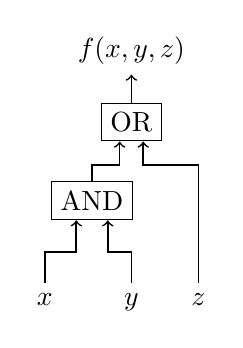
\begin{tikzpicture}
    \node(AND) at (0,1) [rectangle,draw=black] {AND};
    \node (OR) at (.5,2) [rectangle,draw=black] {OR};
    \draw[<-,semithick] (-.2,.75) |- +(-.4,-.4) -- +(-.4,-.8) node[below] {$x$};
    \draw[<-,semithick] (.2,.75) |- +(+.3,-.4) -- +(+.3,-.8) node[below] {$y$};
    \draw[<-,semithick] (0.35,1.75) -- +(0,-.3) -| (AND);
    \draw[<-,semithick] (0.65,1.75) -- +(0,-.3) -| +(.7,-1.8) node[below] {$z$};
    \draw[->,semithick] (OR) -- +(0,0.6) node[above] {$f(x,y,z)$};
  \end{tikzpicture}
  \caption{Circuit computing $f(x,y,z)=(x\wedge y)\vee z$. Note that this (simple) circuit satisfies the requirements we proposed: No circuits, only gates having two inputs and exactly one output.}
  \label{fig:simple-circuit}
\end{figure}

The function $f$ can -- and will -- be represented straightforwardly by the circuit $C$ shown in Figure \ref{fig:simple-circuit}. This circuit simply consists of two gates (and some wires connecting these gates properly), one of which is computing the AND of $x$ and $y$, the other one taking the OR of $z$ and the result given by the AND-gate. This circuit is deliberately simply for illustration purposes, but the concepts extend to more complicated circuits\footnote{As long as they have a certain structure (see \ref{sec:original-circuit-suitable-format})}.

Remember now that we want to compute $f(x,y,z)$ in a way such that no participant can infer more information about the inputs than the result $f(x,y,z)$ itself implicitly reveals. Since we want \emph{no} participant to gather information about the inputs of the other two players, it is not a good idea to leave the whole computation to one participant alone. Thus, we will compute the function \emph{collaboratively} and thereby take care that no participant has to reveal his input to some other participant.

However, if we operate \emph{directly} on the given circuit, our participants would have to supply their inputs without obfuscation (or something similar) so that the participants could see each others' inputs. That's why we resort to a \emph{garbled circuit}.

\subsubsection{The idea of a  garbled circuit.}

As said above, to compute $f(x,y,z)$, we first construct a ``garbled circuit''. Note that when we evaluate the circuit $C$ (the one depicted in Figure \ref{fig:simple-circuit}) for some inputs $x$, $y$ and $z$, each wire has a certain value (0 or 1) that we call the wire's \emph{semantics}. These semantics are represented by a special \emph{signal} (the semantic $\mathbf{0}$ is represented by the signal $0$, while semantic $\mathbf{1}$ is represented by signal $1$). Once we supply the inputs to circuit $C$, all its internal semantics are known (or can be computed easily).

It is important that we can differentiate between the \emph{semantics} and the \emph{signal} of a wire. In ``normal life'' (i.e. when we evaluate circuits without restrictions on privacy of inputs), we will -- for simplicity and convenience -- associate signals that represent the semantics in some straight-forward way (e.g. signal $0$ represents semantic $\mathbf{0}$). But as we are especially interested in keeping information private, it should be clear that this might exactly be something that we do \emph{not} want here!

That is, we could camouflage the semantics by using signals that cannot easily be mapped onto semantics. Therefore, we might even choose something different than ``single letters'' as signals, but whole strings. When doing so, we want to keep the mapping from signals to semantics (and vice versa) secret. That is, we allow (possibly more complicated) signals across the wires, and associate certain signals with semantics 0, and other signals with semantics 1. However, it shall -- essentially -- \emph{not} be possible that any participant can deduce the semantics from the signals (except for the output wire, where we particularly want to be able to retrieve the semantics, since it represents the function value). On the other hand, it \emph{shall} be possible, that the participants can correctly compute the signals needed for evaluation --- despite not knowing the semantics.

Even if this looks like an impossible task, we remember that we proposed several auxiliary techniques in section \ref{sec:building-blocks-for-the-protocol} that \emph{might} help us to achieve or goal. We will later see how they concretely do so.

\subsubsection{Signals and semantics by example.}
\label{sec:signals-semantics-by-example}

We said that we map signals to semantics (and implicitly vice versa). Now, for example, a wire $\omega$ might ``hold'' signal 010001001 (note that this signal consists of several bits, i.e. a whole bit string), and we map this signal (secretly) to 0. This means, if we see that wire $\omega$ holds this signal, this means that it carries semantics 0 (but we possibly don't know this --- we just know the \emph{signal}).

Note that the same signal (010001001) might be mapped to 1 on another wire $\omega'$, i.e. we map signals to semantics for each wire\footnote{This might be needed if we have more wires than signals available.}. The idea is now, that for all wires but the output wire, we don't publish the mappings between signals. Only the output wire's\footnote{Here we are talking about the output wire of the whole circuit (and not of one single gate).} mappings between signals and semantics are known, since we want to be able to compute the output.

\begin{figure}[t]
  \centering
  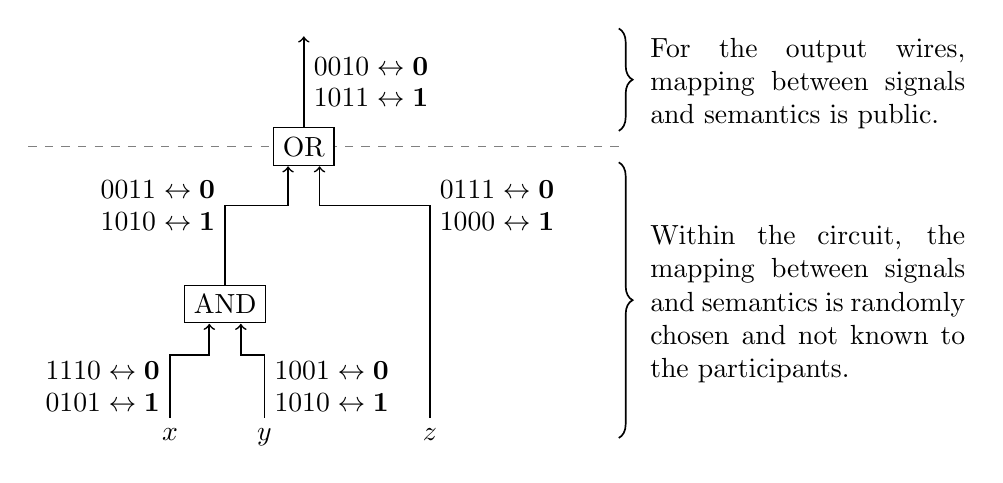
\begin{tikzpicture}
    \node (AND) at (0,1) [rectangle,draw=black] {AND};
    \node (OR) at (1,3) [rectangle,draw=black] {OR};
    % x->AND
    \draw[<-,semithick] (-.2,.75) |- +(-.5,-.4) -- 
      node[yshift=2mm,left] {$1110\leftrightarrow \mathbf{0}$} 
      node[yshift=-2mm,left] {$0101\leftrightarrow \mathbf{1}$} 
    +(-.5,-1.2) node[below] {$x$};
    % y->AND
    \draw[<-,semithick] (.2,.75) |- +(+.3,-.4) -- 
      node[yshift=2mm,right] {$1001\leftrightarrow \mathbf{0}$} 
      node[yshift=-2mm,right] {$1010\leftrightarrow \mathbf{1}$} 
    +(+.3,-1.2) node[below] {$y$};
    % AND->OR
    \draw[<-,semithick] (.8,2.75) |- +(-.8,-.5) 
       node[yshift=2mm,left] {$0011\leftrightarrow \mathbf{0}$ }
       node[yshift=-2mm,left] {$1010\leftrightarrow \mathbf{1}$ } --
    (AND);
    % z->OR
    \draw[<-,semithick] (1.2,2.75) |- ++(+1.4,-.5) 
      node[yshift=2mm,right] {$0111\leftrightarrow \mathbf{0}$} 
      node[yshift=-2mm,right] {$1000\leftrightarrow \mathbf{1}$} --
    +(0,-2.7) node[below] {$z$};
    % OR->output
    \draw[->,semithick] (OR) -- 
      node[yshift=2mm,right] {$0010\leftrightarrow \mathbf{0}$} 
      node[yshift=-2mm,right] {$1011\leftrightarrow \mathbf{1}$} 
    +(0,1.4);
    % legend
    \draw[dashed,gray](-2.5,3) -- (0.6,3);
    \draw[dashed,gray](5,3) -- (1.4,3);
    \draw[decoration={brace,amplitude=0.5em},decorate,semithick] (5,4.5)--(5,3.2);
    \draw[decoration={brace,amplitude=0.5em},decorate,semithick] (5,2.8)--(5,-.7);
    \node[text width=4cm,text justified] () at (7.4,1) {
      Within the circuit, the mapping
      between signals and semantics is
      randomly chosen and not
      known to the participants.};
    \node[text width=4cm,text justified] () at (7.4,3.8) {
      For the output wires, mapping between signals and semantics is public.
    };
  \end{tikzpicture}
  \caption{Associating random signals with semantics. The input wire for variable $y$ associates signal $1001$ with semantics $\mathbf{0}$ and signal $1010$ with semantics $\mathbf{1}$. While all input and internal signals and semantics cannot be mapped onto each other, the signals and semantics of the \emph{output} wire are constructed in such a way that the signal's last bit coincides with the desired semantics. Note that the ``structure'' (i.e. placement of gates and wires) of the garbled circuit corresponds to that of the original circuit depicted in Figure \ref{fig:simple-circuit}.}
  \label{fig:associating-random-signals-with-actual-semantics}
\end{figure}

We come now back to our circuit $C$ and ``install the new signals'': Therefore, we ``remove the original signals'', and replace them by new (random) signals that are mapped onto semantics. We illustrate this concept in Figure \ref{fig:associating-random-signals-with-actual-semantics}. In our example, we see, that if the left incoming wire of the AND-gate holds signal 0101 (representing semantics \textbf{1}), and if the right incoming wire of the AND-gate holds 1001 (representing semantics \textbf{0}), we should get the output signal 0011 (representing semantics $\mathbf{0}=\mathbf{1}\wedge \mathbf{0}$).

Only the output wire's association between semantics and signals (i.e. $0010\leftrightarrow \mathbf{0}$ and $1011\leftrightarrow \mathbf{1}$) is publicly known. They are constructed such that the last digit of the signal corresponds to the desired semantics. This is useful since we want all participants to simply be able to deduce the functions outcome from the output wires of the circuit.

All \emph{internal} mappings from signals to semantics, are unknown to the participants. Please note the difference between the fact that the relation between internal signals and semantics is properly \emph{defined}, and the fact that they are \emph{not known} to the players. This is a central point for the protocol to work.

\paragraph{In a nutshell: What is our goal?}

We later want something like the following: Each player shall get the garbled circuit, and \emph{only} the input signals (also in garbled format). From these, each player shall be able to compute the output values of the circuit. This is depicted in figure \ref{fig:sample-computation}. On the way to this, the player shall not be able to deduce the semantics of input or intermediate wires\footnote{If some player supplies some input, she of course knows the semantics of the corresponding input wire. We just want to ensure that no player learns the semantics of inputs that are not supplied by herself.}.

Moreover, if a player has computed e.g. the even signal for a wire, she should not be able to deduce the odd signal for that wire.

\begin{figure}[t]
  \centering
  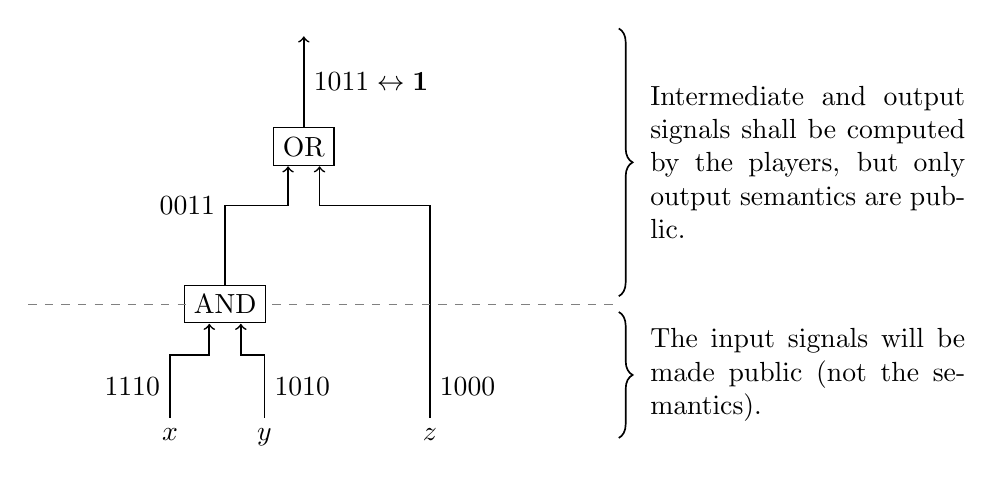
\begin{tikzpicture}
    \node (AND) at (0,1) [rectangle,draw=black] {AND};
    \node (OR) at (1,3) [rectangle,draw=black] {OR};
    % x->AND
    \draw[<-,semithick] (-.2,.75) |- +(-.5,-.4) -- 
      node[left] {$1110$} 
    +(-.5,-1.2) node[below] {$x$};
    % y->AND
    \draw[<-,semithick] (.2,.75) |- +(+.3,-.4) -- 
      node[right] {$1010$} 
    +(+.3,-1.2) node[below] {$y$};
    % AND->OR
    \draw[<-,semithick] (.8,2.75) |- +(-.8,-.5) 
       node[left] {$0011$ } --
    (AND);
    % z->OR
    \draw[<-,semithick] (1.2,2.75) |- ++(+1.4,-.5) 
      node[yshift=-2.3cm,right] {$1000$} --
    +(0,-2.7) node[below] {$z$};
    % OR->output
    \draw[->,semithick] (OR) -- 
      node[right] {$1011\leftrightarrow \mathbf{1}$} 
    +(0,1.4);
    % legend
    \draw[dashed,gray](-2.5,1) -- (-.5,1);
    \draw[dashed,gray](.6,1) -- (5,1);
    \draw[decoration={brace,amplitude=0.5em},decorate,semithick] (5,4.5)--(5,1.1);
    \draw[decoration={brace,amplitude=0.5em},decorate,semithick] (5,.9)--(5,-.7);
    \node[text width=4cm,text justified] () at (7.4,.1) {
      The input signals will be made public (not the semantics).
      };
    \node[text width=4cm,text justified] () at (7.4,2.8) {
      Intermediate and output signals shall be computed by the players, 
      but only output semantics are public.
    };
  \end{tikzpicture}
  \caption{Our goal: The players shall -- given a garbled circuit and garbled inputs -- compute intermediate and output signals. From the output signals, they can deduce the output of the function. This example shows the garbled inputs for $x=\mathbf{0}, y=\mathbf{1}, z=\mathbf{1}$ (see figure \ref{fig:associating-random-signals-with-actual-semantics} for reference). The players shall not be able to deduce the other signals for the wires. Since $f(0,1,1) = (0\wedge 1) \vee 1 = 1$, each player shall -- at last -- learn the output signal $1011$ which stands for semantics $\mathbf{1}$.}
  \label{fig:sample-computation}
\end{figure}


\paragraph{Format of the signals.}

Note that all signals have the same length and are binary strings. Moreover, it is worth noting that for each wire, exactly one signal is ending in 1, while the other is ending in 0. We call the signals ending in 0 ``even signals'' and the signals ending in 1 ``odd signals'' (for obvious reasons). Even if we don't strictly need this convention, it is quite helpful and makes notational issues a bit easier.

Since we want to collaboratively compute the circuit, it should not be the case that e.g. one single player has to define all the signals, and possibly declare his defined signal public. We rather choose some method where all signals are composed of parts supplied by \emph{all} participating parties. To be precise, we require that each party contributes $k$ bits to each signal ($k$ denoting the security parameter). Moreover, we want to construct the signals randomly, since we wanted that concluding the semantics from a signal is not possible (for internal and input wires).

If each of the $n$ players contributes $k$ bits, these are $nk$ bits. To these bits, we add one single bit (again collaboratively randomly chosen) indicating whether it is the even or odd signal (the so-called \emph{parity}). These, in turn, makes signals of length $nk+1$.

Having this construction in mind, we can interpret a signal (i.e. a bit string) of length $nk+1$ as a concatenation of $n$ bit strings each having length $k$ and one last bit to determine whether the signal is odd or even.

So, the only remaining (but very central) question is: ``How can we assure that the intermediate values (i.e. the internal signals) are computed correctly, even if we don't know the association between signals and semantics?''

\paragraph{How can signals propagate along the gates?}
\label{sec:how-can-signals-propagate}

In order to compute the final output value, we will have to determine the output wire's signal (and -- since for this wire we know the mapping -- its semantics). Therefore, we have to compute internal signals along the wires.

To do this, we employ an auxiliary table for each single gate that helps us computing the gate's functionality. We denote the gate's functionality by the symbol $\otimes$ (i.e. the symbol $\otimes$ represents e.g. OR, AND, XOR, NAND or another binary function on bits). This auxiliary table holds four (binary) strings, each of which has length equal to the length of the signals. We construct these bit strings for each gate $g$ and call them call them $A_{00}^g,A_{01}^g,A_{10}^g$ and $A_{11}^g$ (we use superscript $g$ to specify the gates for which the strings are used). 

So, we get a table consisting of 4 rows for a gate taking two inputs and having one output. Remember that we assumed our circuit consisting only of gates with two inputs. Since each input wire can carry either an odd or an even signal, that makes 4 possibilities for the input semantics in total.

As you might guess, that every single entry of these 4 entries in the table is used for one specific computation of the gate, i.e. for one specific combination of odd and even signals along the input wires. For example, if the two input wires of gate $g$ are even, we have to use $A_{00}^g$. If the left incoming wire of gate $g$ carries an odd signal, and the right incoming of gate $g$ carries an even signal, we have to use $A_{01}^g$ for the computation. That is, one has to consider the last bits of the signals carried by the two incoming wires, and choose the value from the table accordingly.

But what do the values of this table ($A^g_{00},A^g_{01},A^g_{10}$ and $A^g_{11}$) look like? Note that we said that the length of a signal is $nk+1$. In order to understand how the table works, we interpret a single signal as $n$ strings, each of length $k$, i.e. we split up the signal into several pieces. Note that, since the length of a signal was $nk+1$, we discard the last bit when doing so.

As we mentioned before, we consider one signal (of length $nk+1$) as $n$ binary strings of length $k$ and one additional parity bit (telling us whether the signal is odd or even). We now split up an incoming signal into $n$ strings of length $k$ and issue each of these strings as input to a pseudorandom generator $G$. This pseudorandom generator (taking a string of length $k$) stretches this input into a longer (binary) string (of length equal twice the length of one single garbled signal). This longer string is then split up into two halves that we call $G_0(s)$ and $G_1(s)$ (for the ``zeroth'' and the ``first'' half of the generator's output).

Depending on the parity on the incoming signal, we either use $G_0$ or $G_1$. If the incoming signal is even, we use $G_0$, while we use $G_1$ if the incoming signal is odd. That is, we split up the signal into $n$ bit strings, feed each of them into a random generator and use the respective halves of the outputs generated by the calls to our random generator $G$. We will come back to that later in more detail (i.e. we will explain how long the output of $G$ is exactly, and which pieces exactly are given to $G$ as inputs). 

That essentially means: For a given even signal (i.e. a signal ending in 0), we compute $G_0(s)$ for all pieces $s$ obtained by splitting up the signal. We proceed analogue for odd signals.

We take then the bit-wise exclusive-or (XOR) of all the values obtained by the pseudorandom generators and the appropriate table entry.

So, let us for now assume that we are considering -- for a certain gate -- the following input signals (for left and right input wire, respectively):

\begin{equation*}
  \sigma=\sigma_1\dots\sigma_na  \quad \text{ and }\quad \tau=\tau_1\dots\tau_nb.
\end{equation*}

That is, each $\sigma_i$ is a bit string of length $k$ and the signal $\sigma$ has parity $a$. Analogously the input signal $\tau$ consists of $n$ parts having length $k$ each (the single $\tau_i$). Then, we later want to be able to compute the gate's output as follows:

\begin{equation}
\label{eq:definition-of-output-of-a-gate-dependent-of-gate-label}
  output \gets G_b(\sigma_1)\oplus\dots\oplus G_b(\sigma_n) \ \oplus \ G_a(\tau_1)\oplus\dots\oplus G_a(\tau_n) \ \oplus \ A_{ab}^g
\end{equation}

You can treat the arrow-sign ($\gets$) as an equality sign. We just chose this symbol here, because we wanted to emphasize that the output \emph{is computed} from some other values. That is, we have to consider all input signals (i.e. all combinations of odd/even signals for this gate) and compute the corresponding table entry $A_{ab}^g$

Let us now think for a moment, why we exactly want to define the output like this: 

In the above equation, $output$ denotes the proper desired result for the specific gate. It should not be overly difficult to solve the above equation (resp. definition) for $A_{ab}^g$ (remark: $a$ and $b$ were the parities of the input signals $\sigma$ and $\tau$, respectively). 

If we do so, we can derive how to construct the values $A_{00}^g,A_{01}^g,A_{10}^g$ and $A_{11}^g$ (by substituting $a$ and $b$ by appropriate values). We now solve equation (\ref{eq:definition-of-output-of-a-gate-dependent-of-gate-label}) for $A_{ab}^g$:

\begin{equation}
  \label{eq:gate-label-definition-with-output}
  A_{ab}^g = G_b(\sigma_1)\oplus\dots\oplus G_b(\sigma_n) \ \oplus \ G_a(\tau_1)\oplus\dots\oplus G_a(\tau_n) \ \oplus \ output
\end{equation}

Even if this beast doesn't look that nice to us (and even if we didn't specify the term $output$ exactly in the above equation), we already now see the following: Equation (\ref{eq:gate-label-definition-with-output}) consists essentially of terms obtained by a random generator (these are the terms $G_b(\sigma_i)$ and $G_a(\tau_j)$) and one term $output$ that are XORed to obtain the result $A_{ab}$. Remember: In section \ref{sec:building-blocks-for-the-protocol} we talked about collaboratively evaluating the XOR-function. We said that we can do this in a constant number of rounds with polynomial amount communication. That means: If we know how to compute the term $output$, we can evaluate this huge XOR in a constant number of rounds with only communication only.

What you should recognize is the following: Equation (\ref{eq:gate-label-definition-with-output}) seems to contain no parametrization that ``adjusts'' the value $A_{ab}$ to the kind of gate that the value will later be used for. This information is contained in the term $output$. Let us now see what this term is looks like exactly.

Remember that the term $output$ should contain the result that one gets when evaluating the considered gate with inputs $\sigma$ and $\tau$, respectively. To be a bit more precise, $output$ shall represent the signal that is ``returned'' by the gate for the given inputs.

Remember that we assigned signals \emph{to each wire}, i.e. in particular to the output wire of the gate we're considering. Moreover, the left input wire holds the signal $\sigma_a$ (i.e. a signal with parity $a$) and the right input wire holds the signal $\tau_b$ (i.e. a signal with parity $b$). As we stated before, for each wire, each of the two signals represents exactly one semantic ($\mathbf{0}$ or $\mathbf{1}$). We now want the following: We want to determine the correct outgoing signal such that the \emph{semantics} associated with the computed outgoing signal are the same as the \emph{semantics} we would obtain if we would map $\sigma_a$ and $\tau_b$ onto their respective semantics and evaluate the ungarbled (i.e. the original) gate for these input semantics. That is we essentially want to know: ``What would the original gate return on inputs represented by the semantics of the input wires?'' The obvious problem here is of course, that we do not know the mapping between signals and semantics, and we just have the signals.

Surprisingly, it is still possible to properly compute the outgoing signal such that its associated semantics represent the desired computation! 

\paragraph{How to compute the value of the variable $output$.}
\label{sec:how-compute-value-variable-output}

Before we go on, we need some additional definitions. First of all, let us give names to these wires: We call the input wires $\alpha$ and $\beta$ (carrying signals $\sigma$ and $\tau$, respectively), and we call the outgoing wire $\gamma$ (will then carry the signal we want to compute).

Let us call the even and odd signals for the gate's output wire $s^\gamma_0$ and $s^\gamma_1$, respectively (remember: these are just signals, and we do not know the mapping to the associated semantics). That is, when we want to compute the gate's output, we have to decide whether we choose $s^\gamma_0$ or $s^\gamma_1$ as the resulting signal. So, essentially, we have to compute the subscript index.

\newcommand{\semoutput}{\lambda}

Moreover, we will need the \emph{semantics} for the incoming wires and outgoing wire. 

We will now need a single bit for each of these three wires -- for now called $\semoutput_\alpha,\semoutput_\beta,\semoutput_\gamma\in\left\{ 0,1 \right\}$ -- that defines for the corresponding wire whether the even signal is associated with semantics $\mathbf{0}$ or vice versa. The subscript denotes the wire that is associated with that bit.

That is, if e.g. $\semoutput_\alpha=0$ (this bit is of course for wire $\alpha$), we -- on this wire -- associate the even signal with semantics $\mathbf{0}$ and the odd signal with $\mathbf{1}$. If $\semoutput_\alpha=1$, it is just the other way around\footnote{The bit $\semoutput$ basically tells us how we can construct the semantics from the last bit of the outgoing signal.}. As you can see, one single bit suffices to fully define the semantics of a wire.

Note that using this bit, one can easily compute the semantics from a signal (for a specific wire). We simply take the last bit of the signal (the parity bit) and XOR it with the corresponding bit $\semoutput$ for this wire.

\begin{equation}
  \label{eq:output-straight-definition-in-informal-part}
  output := s^\gamma_{ \left[ (\semoutput_\alpha \oplus a) \otimes (\semoutput_\beta \oplus b)\right]  \oplus \semoutput_\gamma}
\end{equation}

So, why does this make sense? Consider for now, just the subscript index
\begin{equation*}
\left[ (\semoutput_\alpha \oplus a) \otimes (\semoutput_\beta \oplus b)\right]  \oplus \semoutput_\gamma
\end{equation*}
and take it to pieces:

The term $(\semoutput_\alpha \oplus a)$ is the \emph{semantics} carried by the input wire $\alpha$ (we said that we can compute the semantics by taking the XOR of the $\semoutput$-variable with appropriate index -- in this case $\alpha$ -- and the parity bit, which is -- in this case -- $a$). Analogously, $(\semoutput_\beta \oplus b)$ is the semantics carried by input wire $\beta$.

Remember that we are considering one particular gate that computes the function denoted by the symbol $\otimes$. Thus, $(\semoutput_\alpha \oplus a)\otimes (\semoutput_\beta \oplus b)$ is exactly the semantics that we expect to obtain on wire $\gamma$ when we would evaluate the original gate. Thus, if we want to have the associated signal to that semantics, we have to reconstruct it by XORing this value with $\semoutput_\gamma$.

That is, if we define $output$ this way, it gives us \emph{exactly} the signal we need for the output wire.

Moreover note that we said that it is possible to evaluate a circuit with bounded fan in and depth $d$ in $O(d)$ rounds with polynomial communication. Note that the circuit needed to compute this subscript has bounded fan-in and constant depth, thus can be computed in $O(1)$ rounds.

It remains to clear how the values $\semoutput_\alpha,\semoutput_\beta$ and $\semoutput_\gamma$ are constructed. Again, since we do not want any participant to compute something alone, we construct these values collaboratively. Therefore, the participants generate random bits and take the XOR of them. Again, this is a collaborative evaluation of the XOR function which -- as we know -- can be evaluated in a constant number of rounds with polynomial communication amount.

But when one considers equation (\ref{eq:gate-label-definition-with-output}), one might ask why we XOR this value with all the outputs generated by some pseudorandom generators. This is exactly what prevents all participants from determining the mapping between signals and semantics: If we generate the gate labels using pseudorandom generators, no one can conclude the mapping between signals and semantics, since it is scrambled (for a bit more on this, please consult section \ref{sec:appendix-why-pseudorandom-generators}). 

So far, we have seen how we can compute the output \emph{signal} of a certain gate, given its input signals (not its input \emph{semantics}). That way, we can ``go through'' the circuit and evaluate one gate after another, finally arriving at the gates whose outgoing wires represent the functions output value.

If we now want to compute our original function, we can just evaluate the circuit associated with proper inputs. Since the mappings from from signals to semantics are known for the output wires, we can reconstruct the solution representing our function value.

%%% Local Variables: 
%%% mode: latex
%%% TeX-master: "seminar"
%%% End: 